subsection{Regression}
The objective of the regression task is to perform localization with performance comparable to GPS system.

The parameters of the training had to be tuned for the Network to perform at its best for the regression task.

The layer of the network are initialized using normal distributions. The initialization variances had to be changed so that the weights are big enough to propagate information through the Network while still ensuring convergence.
The initial learning rate and its evolution policy heavily depends on the loss used. For the regression task the initial learning rate was limited by the initial loss.

Based on those general settings, we tested three different approaches. The first one consists in testing those parameters uniformly among the network. The second one consists in fine-tuning the learning rate of each layer differently. The third one consists in loading the weights of the convolution layers from the classification training. In order to compare our results with those three approaches, we refer to the following loss function :

\begin{equation} 
Loss = \frac{0.5}{scale^{2}}*\sum_{i=1,\ 4}(label_{i}-prediction_{i})^{2}}
\end{equation}

The first approach allowed to achieve an average error of 19.3 meters per label as it is shown in the Figure 1a. However after the training, the convolution layers filters did not exhibit any specific features. Thus, it appears that the regression was only supported by the fully connected layers. In our case where the goal is to build a seasonal invariant representation of natural scenes this approach did not reach our expectations. 
*** reference figure Test 26 193

The second approach led us to consider the difference of behavior of the fully-connected layers regarding the sensitivity to learning rate. By decreasing the learning rate of those layers, we forced the convolution layers to take part in the regression. This method resulted in being more successful than the previous one. The best average error we achieved is 18.3 meters. Some natural environment features can be retrieved in the convolution filters.
*** reference figure Test 37 191

The last approach was used on the first approach configuration. It was observed that the convolution weights decreased during the training and lasted with the same order of distribution than with the previous approaches. However the convolution filters retrieved exhibited different structure than the previous approach.
*** reference figure Test 30 191

\begin{figure}[ht]
\centering
\begin{subfigure}{0.33\textwidth}
\centering
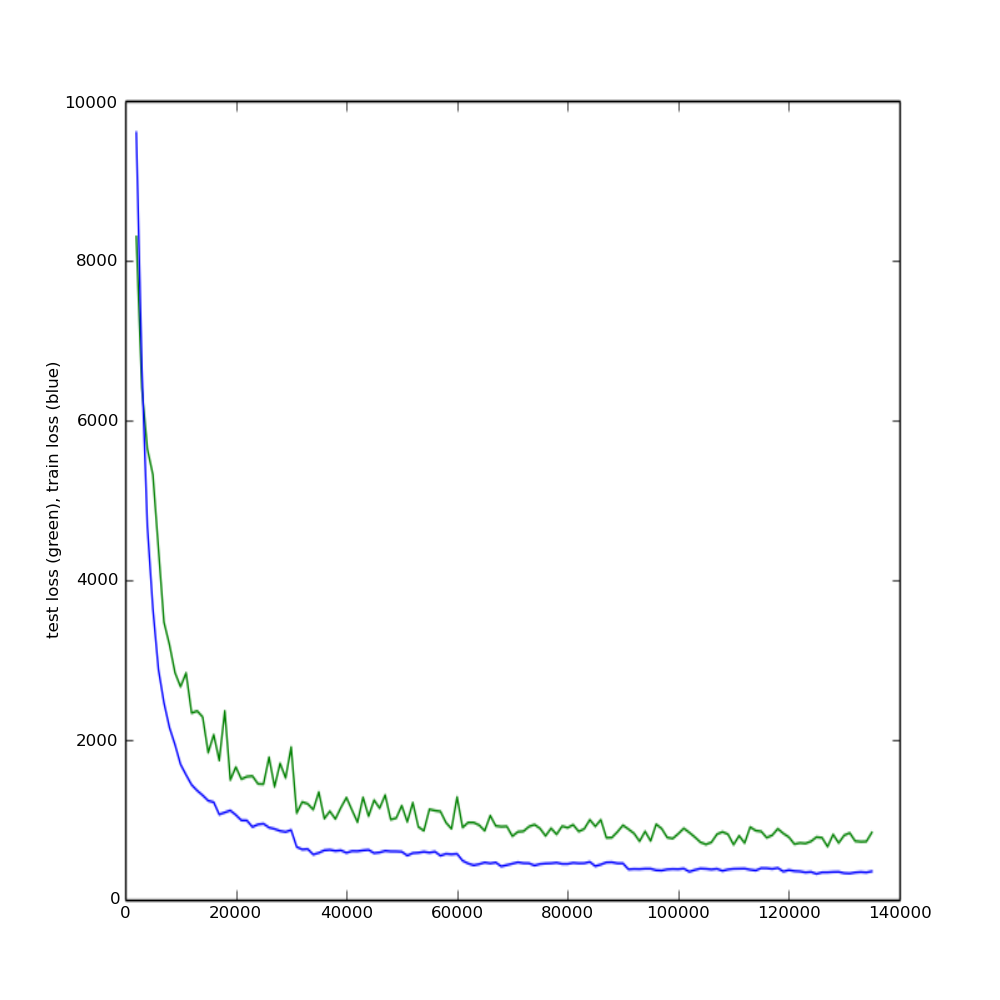
\includegraphics[width=0.9\linewidth]{images/regression/test_loss_26_135000.png}
\caption{First apparoach}
\end{subfigure}%
\begin{subfigure}{0.33\textwidth}
\centering
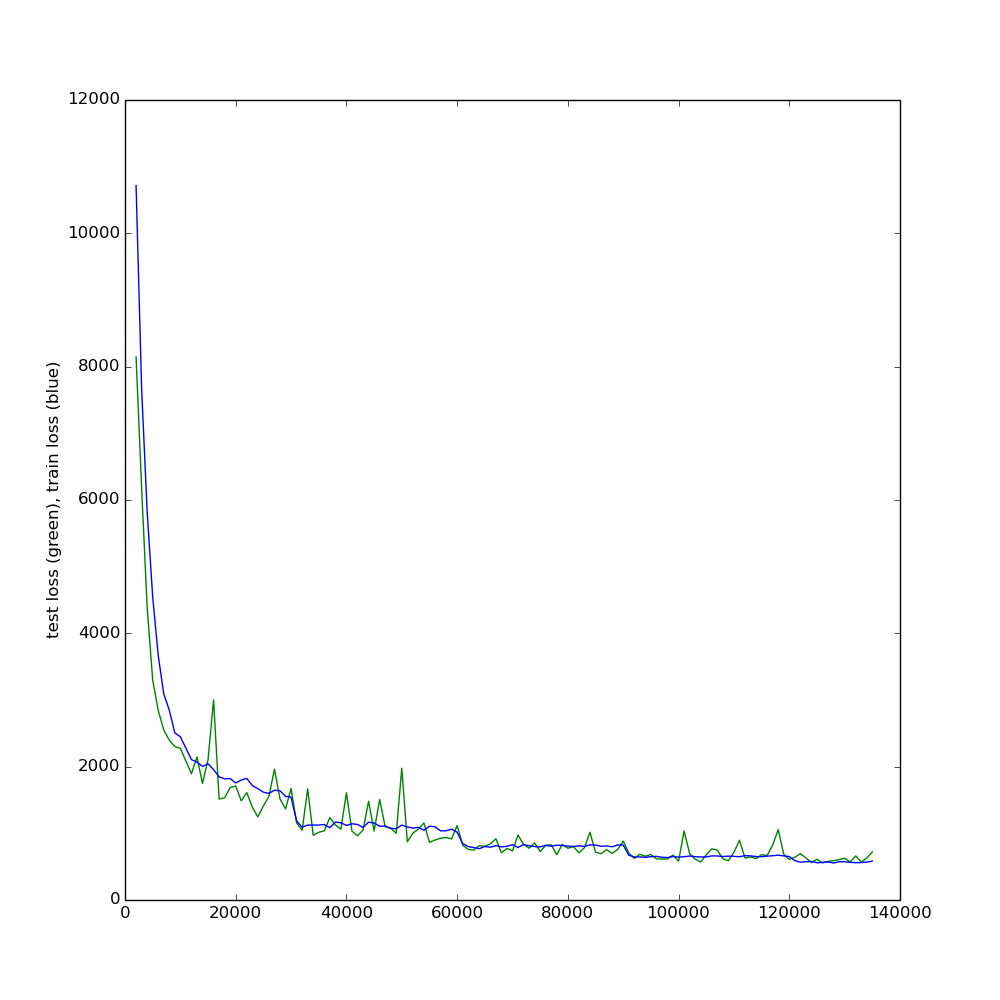
\includegraphics[width=0.9\linewidth]{images/regression/test_loss_37_135000.png}
\caption{Second apparoach}
\end{subfigure}%
\begin{subfigure}{0.33\textwidth}
\centering
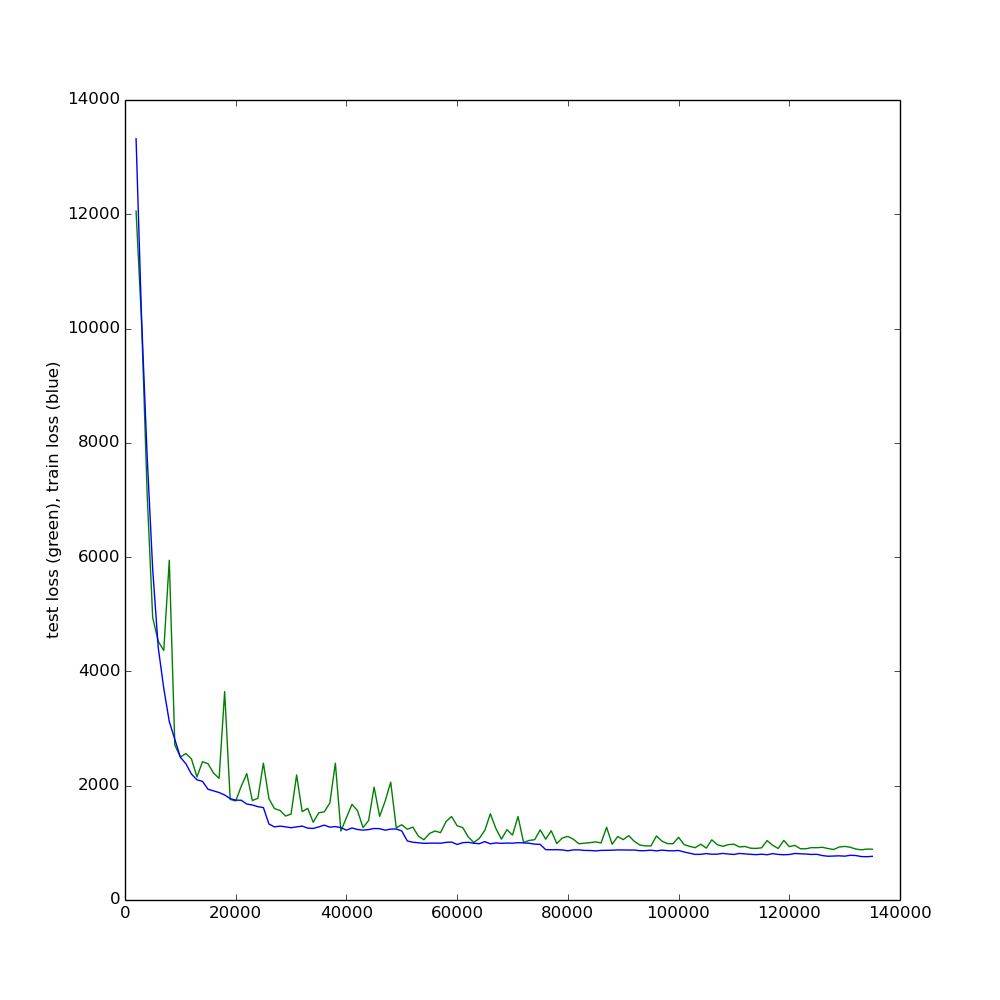
\includegraphics[width=0.9\linewidth]{images/regression/test_loss_30_135000.png}
\caption{Third apparoach}
\end{subfigure}
\caption{Loss Function for 135 000 iterations}
\end{figure}

\begin{figure}[ht]
\centering
\begin{subfigure}{0.33\textwidth}
\centering
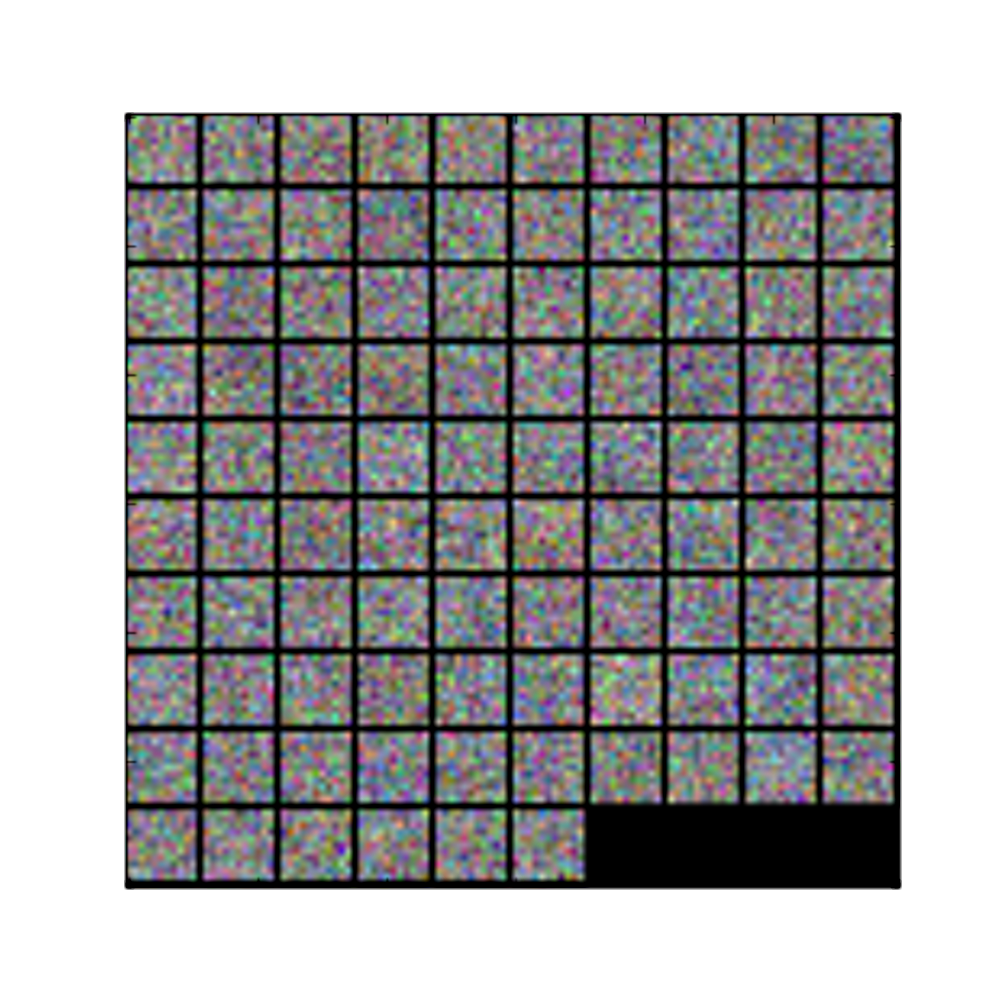
\includegraphics[width=0.9\linewidth]{images/regression/conv1_26_135000.png}
\caption{First apparoach}
\end{subfigure}%
\begin{subfigure}{0.33\textwidth}
\centering
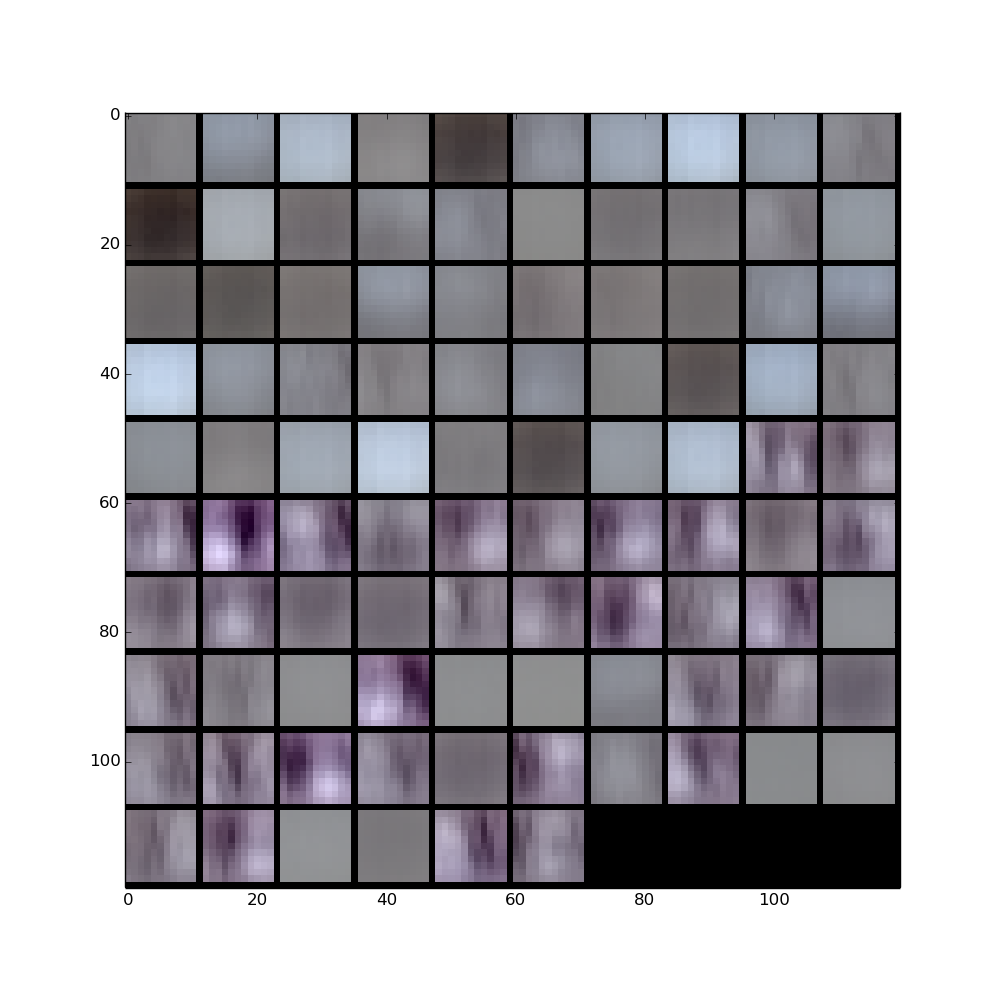
\includegraphics[width=0.9\linewidth]{images/regression/conv1_37_135000.png}
\caption{Second apparoach}
\end{subfigure}%
\begin{subfigure}{0.33\textwidth}
\centering
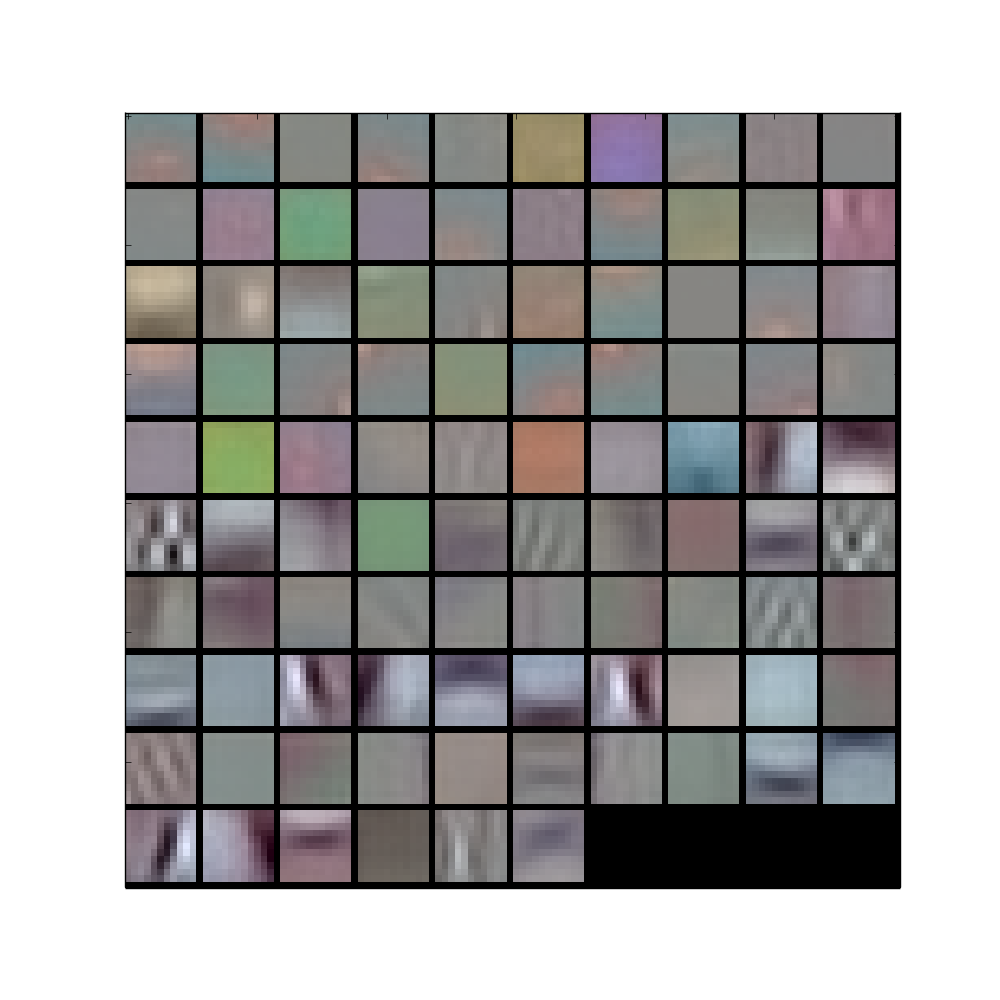
\includegraphics[width=0.9\linewidth]{images/regression/conv1_30_135000.png}
\caption{Third apparoach}
\end{subfigure}
\caption{Conv1 filters after 135 000 iterations}
\end{figure}
